% Created by tikzDevice version 0.12.6 on 2026-07-16 13:12:48
% !TEX encoding = UTF-8 Unicode
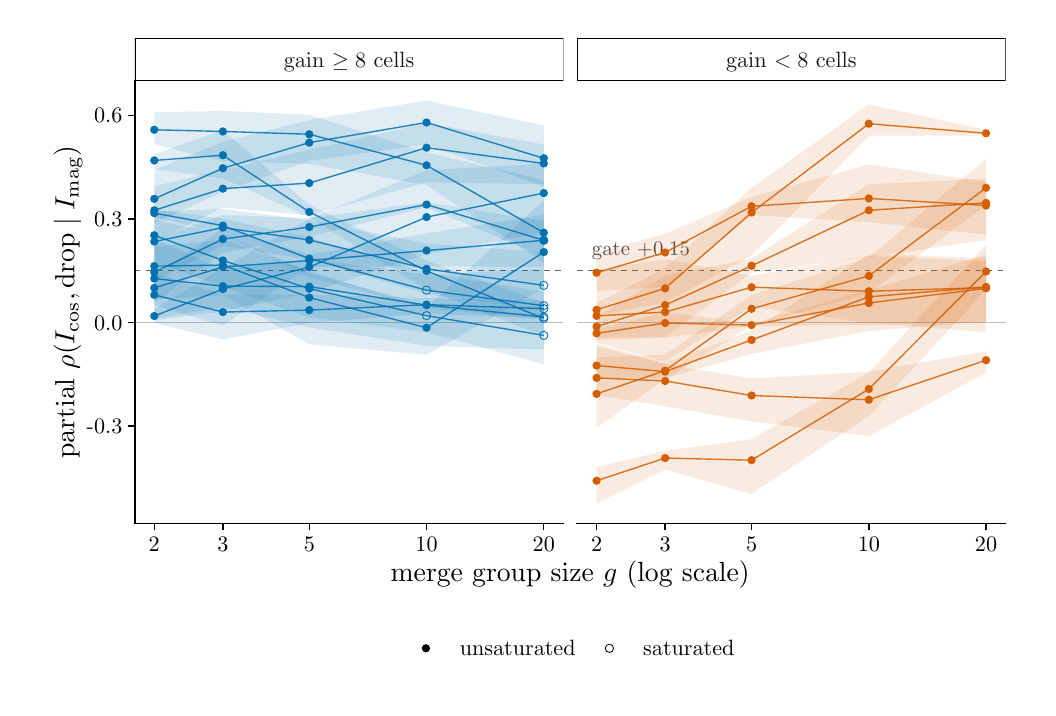
\begin{tikzpicture}[x=1pt,y=1pt]
\definecolor{fillColor}{RGB}{255,255,255}
\path[use as bounding box,fill=fillColor,fill opacity=0.00] (0,0) rectangle (361.35,238.49);
\begin{scope}
\path[clip] (  0.00,  0.00) rectangle (361.35,238.49);
\definecolor{drawColor}{RGB}{255,255,255}
\definecolor{fillColor}{RGB}{255,255,255}

\path[draw=drawColor,line width= 0.5pt,line join=round,line cap=round,fill=fillColor] (  0.00,  0.00) rectangle (361.35,238.49);
\end{scope}
\begin{scope}
\path[clip] ( 38.72, 59.35) rectangle (193.53,219.43);
\definecolor{fillColor}{RGB}{255,255,255}

\path[fill=fillColor] ( 38.72, 59.35) rectangle (193.53,219.43);
\definecolor{drawColor}{gray}{0.40}

\path[draw=drawColor,line width= 0.4pt,dash pattern=on 2pt off 2pt ,line join=round] ( 38.72,150.66) -- (193.53,150.66);
\definecolor{drawColor}{gray}{0.75}

\path[draw=drawColor,line width= 0.3pt,line join=round] ( 38.72,131.94) -- (193.53,131.94);
\definecolor{fillColor}{RGB}{0,114,178}

\path[fill=fillColor,fill opacity=0.12] ( 45.75,149.99) --
	( 70.54,142.08) --
	(101.76,142.04) --
	(144.13,140.74) --
	(186.50,139.87) --
	(186.50,133.43) --
	(144.13,135.18) --
	(101.76,131.76) --
	( 70.54,125.88) --
	( 45.75,131.77) --
	cycle;

\path[] ( 45.75,149.99) --
	( 70.54,142.08) --
	(101.76,142.04) --
	(144.13,140.74) --
	(186.50,139.87);

\path[] (186.50,133.43) --
	(144.13,135.18) --
	(101.76,131.76) --
	( 70.54,125.88) --
	( 45.75,131.77);

\path[fill=fillColor,fill opacity=0.12] ( 45.75,162.11) --
	( 70.54,151.22) --
	(101.76,154.92) --
	(144.13,149.17) --
	(186.50,151.30) --
	(186.50,122.22) --
	(144.13,123.48) --
	(101.76,130.22) --
	( 70.54,137.62) --
	( 45.75,133.30) --
	cycle;

\path[] ( 45.75,162.11) --
	( 70.54,151.22) --
	(101.76,154.92) --
	(144.13,149.17) --
	(186.50,151.30);

\path[] (186.50,122.22) --
	(144.13,123.48) --
	(101.76,130.22) --
	( 70.54,137.62) --
	( 45.75,133.30);

\path[fill=fillColor,fill opacity=0.12] ( 45.75,168.92) --
	( 70.54,164.19) --
	(101.76,149.90) --
	(144.13,138.28) --
	(186.50,137.06) --
	(186.50,116.86) --
	(144.13,128.42) --
	(101.76,133.78) --
	( 70.54,144.90) --
	( 45.75,154.02) --
	cycle;

\path[] ( 45.75,168.92) --
	( 70.54,164.19) --
	(101.76,149.90) --
	(144.13,138.28) --
	(186.50,137.06);

\path[] (186.50,116.86) --
	(144.13,128.42) --
	(101.76,133.78) --
	( 70.54,144.90) --
	( 45.75,154.02);

\path[fill=fillColor,fill opacity=0.12] ( 45.75,187.07) --
	( 70.54,197.30) --
	(101.76,205.09) --
	(144.13,212.15) --
	(186.50,203.13) --
	(186.50,181.10) --
	(144.13,196.30) --
	(101.76,190.42) --
	( 70.54,179.25) --
	( 45.75,167.84) --
	cycle;

\path[] ( 45.75,187.07) --
	( 70.54,197.30) --
	(101.76,205.09) --
	(144.13,212.15) --
	(186.50,203.13);

\path[] (186.50,181.10) --
	(144.13,196.30) --
	(101.76,190.42) --
	( 70.54,179.25) --
	( 45.75,167.84);

\path[fill=fillColor,fill opacity=0.12] ( 45.75,192.79) --
	( 70.54,201.47) --
	(101.76,174.40) --
	(144.13,154.32) --
	(186.50,139.16) --
	(186.50,127.03) --
	(144.13,143.89) --
	(101.76,169.98) --
	( 70.54,184.05) --
	( 45.75,187.39) --
	cycle;

\path[] ( 45.75,192.79) --
	( 70.54,201.47) --
	(101.76,174.40) --
	(144.13,154.32) --
	(186.50,139.16);

\path[] (186.50,127.03) --
	(144.13,143.89) --
	(101.76,169.98) --
	( 70.54,184.05) --
	( 45.75,187.39);

\path[fill=fillColor,fill opacity=0.12] ( 45.75,172.76) --
	( 70.54,169.41) --
	(101.76,162.72) --
	(144.13,149.95) --
	(186.50,143.01) --
	(186.50,132.93) --
	(144.13,137.15) --
	(101.76,148.25) --
	( 70.54,164.17) --
	( 45.75,170.03) --
	cycle;

\path[] ( 45.75,172.76) --
	( 70.54,169.41) --
	(101.76,162.72) --
	(144.13,149.95) --
	(186.50,143.01);

\path[] (186.50,132.93) --
	(144.13,137.15) --
	(101.76,148.25) --
	( 70.54,164.17) --
	( 45.75,170.03);

\path[fill=fillColor,fill opacity=0.12] ( 45.75,172.03) --
	( 70.54,173.00) --
	(101.76,168.93) --
	(144.13,160.51) --
	(186.50,157.38) --
	(186.50,136.24) --
	(144.13,142.30) --
	(101.76,154.71) --
	( 70.54,159.74) --
	( 45.75,146.84) --
	cycle;

\path[] ( 45.75,172.03) --
	( 70.54,173.00) --
	(101.76,168.93) --
	(144.13,160.51) --
	(186.50,157.38);

\path[] (186.50,136.24) --
	(144.13,142.30) --
	(101.76,154.71) --
	( 70.54,159.74) --
	( 45.75,146.84);

\path[fill=fillColor,fill opacity=0.12] ( 45.75,207.87) --
	( 70.54,208.41) --
	(101.76,207.00) --
	(144.13,193.39) --
	(186.50,183.42) --
	(186.50,153.51) --
	(144.13,181.65) --
	(101.76,189.25) --
	( 70.54,190.31) --
	( 45.75,196.24) --
	cycle;

\path[] ( 45.75,207.87) --
	( 70.54,208.41) --
	(101.76,207.00) --
	(144.13,193.39) --
	(186.50,183.42);

\path[] (186.50,153.51) --
	(144.13,181.65) --
	(101.76,189.25) --
	( 70.54,190.31) --
	( 45.75,196.24);

\path[fill=fillColor,fill opacity=0.12] ( 45.75,181.20) --
	( 70.54,187.08) --
	(101.76,194.39) --
	(144.13,204.01) --
	(186.50,196.24) --
	(186.50,181.92) --
	(144.13,182.61) --
	(101.76,170.63) --
	( 70.54,173.58) --
	( 45.75,161.11) --
	cycle;

\path[] ( 45.75,181.20) --
	( 70.54,187.08) --
	(101.76,194.39) --
	(144.13,204.01) --
	(186.50,196.24);

\path[] (186.50,181.92) --
	(144.13,182.61) --
	(101.76,170.63) --
	( 70.54,173.58) --
	( 45.75,161.11);

\path[fill=fillColor,fill opacity=0.12] ( 45.75,136.87) --
	( 70.54,151.67) --
	(101.76,169.41) --
	(144.13,186.97) --
	(186.50,189.32) --
	(186.50,164.29) --
	(144.13,156.73) --
	(101.76,142.70) --
	( 70.54,136.02) --
	( 45.75,132.73) --
	cycle;

\path[] ( 45.75,136.87) --
	( 70.54,151.67) --
	(101.76,169.41) --
	(144.13,186.97) --
	(186.50,189.32);

\path[] (186.50,164.29) --
	(144.13,156.73) --
	(101.76,142.70) --
	( 70.54,136.02) --
	( 45.75,132.73);

\path[fill=fillColor,fill opacity=0.12] ( 45.75,159.41) --
	( 70.54,161.82) --
	(101.76,150.54) --
	(144.13,137.32) --
	(186.50,175.98) --
	(186.50,144.37) --
	(144.13,120.29) --
	(101.76,124.07) --
	( 70.54,141.83) --
	( 45.75,140.36) --
	cycle;

\path[] ( 45.75,159.41) --
	( 70.54,161.82) --
	(101.76,150.54) --
	(144.13,137.32) --
	(186.50,175.98);

\path[] (186.50,144.37) --
	(144.13,120.29) --
	(101.76,124.07) --
	( 70.54,141.83) --
	( 45.75,140.36);

\path[fill=fillColor,fill opacity=0.12] ( 45.75,161.98) --
	( 70.54,170.77) --
	(101.76,169.69) --
	(144.13,175.34) --
	(186.50,168.67) --
	(186.50,155.82) --
	(144.13,173.61) --
	(101.76,162.92) --
	( 70.54,157.20) --
	( 45.75,139.04) --
	cycle;

\path[] ( 45.75,161.98) --
	( 70.54,170.77) --
	(101.76,169.69) --
	(144.13,175.34) --
	(186.50,168.67);

\path[] (186.50,155.82) --
	(144.13,173.61) --
	(101.76,162.92) --
	( 70.54,157.20) --
	( 45.75,139.04);

\path[fill=fillColor,fill opacity=0.12] ( 45.75,148.43) --
	( 70.54,166.16) --
	(101.76,156.47) --
	(144.13,164.14) --
	(186.50,170.87) --
	(186.50,151.92) --
	(144.13,152.31) --
	(101.76,151.97) --
	( 70.54,130.86) --
	( 45.75,138.26) --
	cycle;

\path[] ( 45.75,148.43) --
	( 70.54,166.16) --
	(101.76,156.47) --
	(144.13,164.14) --
	(186.50,170.87);

\path[] (186.50,151.92) --
	(144.13,152.31) --
	(101.76,151.97) --
	( 70.54,130.86) --
	( 45.75,138.26);
\definecolor{drawColor}{RGB}{0,114,178}

\path[draw=drawColor,draw opacity=0.85,line width= 0.5pt,line join=round] ( 45.75,141.94) --
	( 70.54,135.72) --
	(101.76,136.44) --
	(144.13,138.40) --
	(186.50,136.97);

\path[draw=drawColor,draw opacity=0.85,line width= 0.5pt,line join=round] ( 45.75,147.84) --
	( 70.54,145.09) --
	(101.76,144.93) --
	(144.13,138.21) --
	(186.50,133.97);

\path[draw=drawColor,draw opacity=0.85,line width= 0.5pt,line join=round] ( 45.75,163.47) --
	( 70.54,154.39) --
	(101.76,144.18) --
	(144.13,134.43) --
	(186.50,127.29);

\path[draw=drawColor,draw opacity=0.85,line width= 0.5pt,line join=round] ( 45.75,176.64) --
	( 70.54,187.69) --
	(101.76,196.95) --
	(144.13,204.23) --
	(186.50,191.28);

\path[draw=drawColor,draw opacity=0.85,line width= 0.5pt,line join=round] ( 45.75,190.51) --
	( 70.54,192.41) --
	(101.76,171.91) --
	(144.13,150.61) --
	(186.50,133.43);

\path[draw=drawColor,draw opacity=0.85,line width= 0.5pt,line join=round] ( 45.75,171.48) --
	( 70.54,166.96) --
	(101.76,155.04) --
	(144.13,143.63) --
	(186.50,138.03);

\path[draw=drawColor,draw opacity=0.85,line width= 0.5pt,line join=round] ( 45.75,161.20) --
	( 70.54,166.23) --
	(101.76,161.77) --
	(144.13,151.32) --
	(186.50,145.37);

\path[draw=drawColor,draw opacity=0.85,line width= 0.5pt,line join=round] ( 45.75,201.59) --
	( 70.54,200.98) --
	(101.76,199.98) --
	(144.13,188.75) --
	(186.50,164.41);

\path[draw=drawColor,draw opacity=0.85,line width= 0.5pt,line join=round] ( 45.75,172.50) --
	( 70.54,180.33) --
	(101.76,182.33) --
	(144.13,195.11) --
	(186.50,189.41);

\path[draw=drawColor,draw opacity=0.85,line width= 0.5pt,line join=round] ( 45.75,134.30) --
	( 70.54,144.03) --
	(101.76,151.97) --
	(144.13,170.04) --
	(186.50,178.72);

\path[draw=drawColor,draw opacity=0.85,line width= 0.5pt,line join=round] ( 45.75,152.33) --
	( 70.54,152.69) --
	(101.76,140.96) --
	(144.13,130.07) --
	(186.50,157.40);

\path[draw=drawColor,draw opacity=0.85,line width= 0.5pt,line join=round] ( 45.75,150.14) --
	( 70.54,162.09) --
	(101.76,166.45) --
	(144.13,174.56) --
	(186.50,161.65);

\path[draw=drawColor,draw opacity=0.85,line width= 0.5pt,line join=round] ( 45.75,144.46) --
	( 70.54,152.02) --
	(101.76,154.35) --
	(144.13,157.94) --
	(186.50,161.67);
\definecolor{fillColor}{RGB}{0,114,178}

\path[fill=fillColor] ( 45.75,176.64) circle (  1.50);

\path[fill=fillColor] ( 70.54,187.69) circle (  1.50);

\path[fill=fillColor] (101.76,196.95) circle (  1.50);

\path[fill=fillColor] (144.13,204.23) circle (  1.50);

\path[fill=fillColor] (186.50,191.28) circle (  1.50);

\path[fill=fillColor] ( 45.75,190.51) circle (  1.50);

\path[fill=fillColor] ( 70.54,192.41) circle (  1.50);

\path[fill=fillColor] (101.76,171.91) circle (  1.50);

\path[fill=fillColor] (144.13,150.61) circle (  1.50);
\definecolor{drawColor}{RGB}{0,114,178}

\path[draw=drawColor,line width= 0.3pt,line join=round,line cap=round] (186.50,133.43) circle (  1.50);

\path[fill=fillColor] ( 45.75,171.48) circle (  1.50);

\path[fill=fillColor] ( 70.54,166.96) circle (  1.50);

\path[fill=fillColor] (101.76,155.04) circle (  1.50);

\path[draw=drawColor,line width= 0.3pt,line join=round,line cap=round] (144.13,143.63) circle (  1.50);

\path[draw=drawColor,line width= 0.3pt,line join=round,line cap=round] (186.50,138.03) circle (  1.50);

\path[fill=fillColor] ( 45.75,161.20) circle (  1.50);

\path[fill=fillColor] ( 70.54,166.23) circle (  1.50);

\path[fill=fillColor] (101.76,161.77) circle (  1.50);

\path[fill=fillColor] (144.13,151.32) circle (  1.50);

\path[draw=drawColor,line width= 0.3pt,line join=round,line cap=round] (186.50,145.37) circle (  1.50);

\path[fill=fillColor] ( 45.75,201.59) circle (  1.50);

\path[fill=fillColor] ( 70.54,200.98) circle (  1.50);

\path[fill=fillColor] (101.76,199.98) circle (  1.50);

\path[fill=fillColor] (144.13,188.75) circle (  1.50);

\path[fill=fillColor] (186.50,164.41) circle (  1.50);

\path[fill=fillColor] ( 45.75,172.50) circle (  1.50);

\path[fill=fillColor] ( 70.54,180.33) circle (  1.50);

\path[fill=fillColor] (101.76,182.33) circle (  1.50);

\path[fill=fillColor] (144.13,195.11) circle (  1.50);

\path[fill=fillColor] (186.50,189.41) circle (  1.50);

\path[fill=fillColor] ( 45.75,134.30) circle (  1.50);

\path[fill=fillColor] ( 70.54,144.03) circle (  1.50);

\path[fill=fillColor] (101.76,151.97) circle (  1.50);

\path[fill=fillColor] (144.13,170.04) circle (  1.50);

\path[fill=fillColor] (186.50,178.72) circle (  1.50);

\path[fill=fillColor] ( 45.75,152.33) circle (  1.50);

\path[fill=fillColor] ( 70.54,152.69) circle (  1.50);

\path[fill=fillColor] (101.76,140.96) circle (  1.50);

\path[fill=fillColor] (144.13,130.07) circle (  1.50);

\path[fill=fillColor] (186.50,157.40) circle (  1.50);

\path[fill=fillColor] ( 45.75,150.14) circle (  1.50);

\path[fill=fillColor] ( 70.54,162.09) circle (  1.50);

\path[fill=fillColor] (101.76,166.45) circle (  1.50);

\path[fill=fillColor] (144.13,174.56) circle (  1.50);

\path[draw=drawColor,line width= 0.3pt,line join=round,line cap=round] (186.50,161.65) circle (  1.50);

\path[fill=fillColor] ( 45.75,144.46) circle (  1.50);

\path[fill=fillColor] ( 70.54,152.02) circle (  1.50);

\path[fill=fillColor] (101.76,154.35) circle (  1.50);

\path[fill=fillColor] (144.13,157.94) circle (  1.50);

\path[fill=fillColor] (186.50,161.67) circle (  1.50);

\path[fill=fillColor] ( 45.75,141.94) circle (  1.50);

\path[fill=fillColor] ( 70.54,135.72) circle (  1.50);

\path[fill=fillColor] (101.76,136.44) circle (  1.50);

\path[fill=fillColor] (144.13,138.40) circle (  1.50);

\path[draw=drawColor,line width= 0.3pt,line join=round,line cap=round] (186.50,136.97) circle (  1.50);

\path[fill=fillColor] ( 45.75,147.84) circle (  1.50);

\path[fill=fillColor] ( 70.54,145.09) circle (  1.50);

\path[fill=fillColor] (101.76,144.93) circle (  1.50);

\path[fill=fillColor] (144.13,138.21) circle (  1.50);

\path[draw=drawColor,line width= 0.3pt,line join=round,line cap=round] (186.50,133.97) circle (  1.50);

\path[fill=fillColor] ( 45.75,163.47) circle (  1.50);

\path[fill=fillColor] ( 70.54,154.39) circle (  1.50);

\path[fill=fillColor] (101.76,144.18) circle (  1.50);

\path[draw=drawColor,line width= 0.3pt,line join=round,line cap=round] (144.13,134.43) circle (  1.50);

\path[draw=drawColor,line width= 0.3pt,line join=round,line cap=round] (186.50,127.29) circle (  1.50);
\end{scope}
\begin{scope}
\path[clip] (198.53, 59.35) rectangle (353.35,219.43);
\definecolor{fillColor}{RGB}{255,255,255}

\path[fill=fillColor] (198.53, 59.35) rectangle (353.35,219.43);
\definecolor{drawColor}{gray}{0.40}

\path[draw=drawColor,line width= 0.4pt,dash pattern=on 2pt off 2pt ,line join=round] (198.53,150.66) -- (353.35,150.66);
\definecolor{drawColor}{gray}{0.75}

\path[draw=drawColor,line width= 0.3pt,line join=round] (198.53,131.94) -- (353.35,131.94);
\definecolor{drawColor}{gray}{0.30}

\node[text=drawColor,anchor=base,inner sep=0pt, outer sep=0pt, scale=  0.75] at (221.61,156.18) {gate $+0.15$};
\definecolor{fillColor}{RGB}{213,94,0}

\path[fill=fillColor,fill opacity=0.12] (205.57,150.91) --
	(230.35,154.88) --
	(261.58,148.93) --
	(303.95,155.98) --
	(346.31,154.16) --
	(346.31,128.49) --
	(303.95,131.76) --
	(261.58,137.70) --
	(230.35,117.78) --
	(205.57,124.61) --
	cycle;

\path[] (205.57,150.91) --
	(230.35,154.88) --
	(261.58,148.93) --
	(303.95,155.98) --
	(346.31,154.16);

\path[] (346.31,128.49) --
	(303.95,131.76) --
	(261.58,137.70) --
	(230.35,117.78) --
	(205.57,124.61);

\path[fill=fillColor,fill opacity=0.12] (205.57,124.18) --
	(230.35,117.37) --
	(261.58,128.91) --
	(303.95,156.57) --
	(346.31,155.28) --
	(346.31,132.31) --
	(303.95,128.87) --
	(261.58,120.64) --
	(230.35,111.86) --
	(205.57,111.93) --
	cycle;

\path[] (205.57,124.18) --
	(230.35,117.37) --
	(261.58,128.91) --
	(303.95,156.57) --
	(346.31,155.28);

\path[] (346.31,132.31) --
	(303.95,128.87) --
	(261.58,120.64) --
	(230.35,111.86) --
	(205.57,111.93);

\path[fill=fillColor,fill opacity=0.12] (205.57,123.45) --
	(230.35,116.93) --
	(261.58,111.70) --
	(303.95,114.14) --
	(346.31,121.59) --
	(346.31,113.80) --
	(303.95, 90.92) --
	(261.58, 96.25) --
	(230.35,101.66) --
	(205.57,105.72) --
	cycle;

\path[] (205.57,123.45) --
	(230.35,116.93) --
	(261.58,111.70) --
	(303.95,114.14) --
	(346.31,121.59);

\path[] (346.31,113.80) --
	(303.95, 90.92) --
	(261.58, 96.25) --
	(230.35,101.66) --
	(205.57,105.72);

\path[fill=fillColor,fill opacity=0.12] (205.57,119.33) --
	(230.35,120.31) --
	(261.58,141.88) --
	(303.95,155.42) --
	(346.31,191.15) --
	(346.31,174.50) --
	(303.95,142.59) --
	(261.58,130.80) --
	(230.35,111.48) --
	(205.57, 93.89) --
	cycle;

\path[] (205.57,119.33) --
	(230.35,120.31) --
	(261.58,141.88) --
	(303.95,155.42) --
	(346.31,191.15);

\path[] (346.31,174.50) --
	(303.95,142.59) --
	(261.58,130.80) --
	(230.35,111.48) --
	(205.57, 93.89);

\path[fill=fillColor,fill opacity=0.12] (205.57,134.09) --
	(230.35,148.82) --
	(261.58,155.09) --
	(303.95,181.95) --
	(346.31,183.93) --
	(346.31,161.75) --
	(303.95,155.53) --
	(261.58,149.98) --
	(230.35,126.72) --
	(205.57,126.50) --
	cycle;

\path[] (205.57,134.09) --
	(230.35,148.82) --
	(261.58,155.09) --
	(303.95,181.95) --
	(346.31,183.93);

\path[] (346.31,161.75) --
	(303.95,155.53) --
	(261.58,149.98) --
	(230.35,126.72) --
	(205.57,126.50);

\path[fill=fillColor,fill opacity=0.12] (205.57,129.34) --
	(230.35,135.71) --
	(261.58,131.59) --
	(303.95,143.65) --
	(346.31,156.47) --
	(346.31,132.11) --
	(303.95,131.05) --
	(261.58,130.57) --
	(230.35,126.44) --
	(205.57,125.63) --
	cycle;

\path[] (205.57,129.34) --
	(230.35,135.71) --
	(261.58,131.59) --
	(303.95,143.65) --
	(346.31,156.47);

\path[] (346.31,132.11) --
	(303.95,131.05) --
	(261.58,130.57) --
	(230.35,126.44) --
	(205.57,125.63);

\path[fill=fillColor,fill opacity=0.12] (205.57, 79.68) --
	(230.35, 85.58) --
	(261.58, 89.79) --
	(303.95,113.86) --
	(346.31,159.99) --
	(346.31,143.80) --
	(303.95, 98.11) --
	(261.58, 70.00) --
	(230.35, 78.77) --
	(205.57, 66.63) --
	cycle;

\path[] (205.57, 79.68) --
	(230.35, 85.58) --
	(261.58, 89.79) --
	(303.95,113.86) --
	(346.31,159.99);

\path[] (346.31,143.80) --
	(303.95, 98.11) --
	(261.58, 70.00) --
	(230.35, 78.77) --
	(205.57, 66.63);

\path[fill=fillColor,fill opacity=0.12] (205.57,138.96) --
	(230.35,151.62) --
	(261.58,180.56) --
	(303.95,210.73) --
	(346.31,201.58) --
	(346.31,199.53) --
	(303.95,199.46) --
	(261.58,156.10) --
	(230.35,139.17) --
	(205.57,134.39) --
	cycle;

\path[] (205.57,138.96) --
	(230.35,151.62) --
	(261.58,180.56) --
	(303.95,210.73) --
	(346.31,201.58);

\path[] (346.31,199.53) --
	(303.95,199.46) --
	(261.58,156.10) --
	(230.35,139.17) --
	(205.57,134.39);

\path[fill=fillColor,fill opacity=0.12] (205.57,157.12) --
	(230.35,164.00) --
	(261.58,177.37) --
	(303.95,189.10) --
	(346.31,182.75) --
	(346.31,163.70) --
	(303.95,168.25) --
	(261.58,170.78) --
	(230.35,144.90) --
	(205.57,143.30) --
	cycle;

\path[] (205.57,157.12) --
	(230.35,164.00) --
	(261.58,177.37) --
	(303.95,189.10) --
	(346.31,182.75);

\path[] (346.31,163.70) --
	(303.95,168.25) --
	(261.58,170.78) --
	(230.35,144.90) --
	(205.57,143.30);
\definecolor{drawColor}{RGB}{213,94,0}

\path[draw=drawColor,draw opacity=0.85,line width= 0.5pt,line join=round] (205.57,134.34) --
	(230.35,135.73) --
	(261.58,144.71) --
	(303.95,143.24) --
	(346.31,144.58);

\path[draw=drawColor,draw opacity=0.85,line width= 0.5pt,line join=round] (205.57,116.40) --
	(230.35,114.20) --
	(261.58,125.65) --
	(303.95,141.22) --
	(346.31,144.81);

\path[draw=drawColor,draw opacity=0.85,line width= 0.5pt,line join=round] (205.57,111.94) --
	(230.35,110.81) --
	(261.58,105.57) --
	(303.95,104.04) --
	(346.31,118.33);

\path[draw=drawColor,draw opacity=0.85,line width= 0.5pt,line join=round] (205.57,106.16) --
	(230.35,114.55) --
	(261.58,136.91) --
	(303.95,148.81) --
	(346.31,180.64);

\path[draw=drawColor,draw opacity=0.85,line width= 0.5pt,line join=round] (205.57,130.49) --
	(230.35,138.24) --
	(261.58,152.44) --
	(303.95,172.51) --
	(346.31,175.18);

\path[draw=drawColor,draw opacity=0.85,line width= 0.5pt,line join=round] (205.57,128.03) --
	(230.35,131.77) --
	(261.58,131.02) --
	(303.95,139.01) --
	(346.31,144.30);

\path[draw=drawColor,draw opacity=0.85,line width= 0.5pt,line join=round] (205.57, 74.77) --
	(230.35, 82.97) --
	(261.58, 82.20) --
	(303.95,107.91) --
	(346.31,150.39);

\path[draw=drawColor,draw opacity=0.85,line width= 0.5pt,line join=round] (205.57,136.53) --
	(230.35,144.29) --
	(261.58,171.68) --
	(303.95,203.78) --
	(346.31,200.33);

\path[draw=drawColor,draw opacity=0.85,line width= 0.5pt,line join=round] (205.57,149.94) --
	(230.35,157.25) --
	(261.58,173.96) --
	(303.95,176.78) --
	(346.31,174.23);
\definecolor{fillColor}{RGB}{213,94,0}

\path[fill=fillColor] (205.57,106.16) circle (  1.50);

\path[fill=fillColor] (230.35,114.55) circle (  1.50);

\path[fill=fillColor] (261.58,136.91) circle (  1.50);

\path[fill=fillColor] (303.95,148.81) circle (  1.50);

\path[fill=fillColor] (346.31,180.64) circle (  1.50);

\path[fill=fillColor] (205.57,130.49) circle (  1.50);

\path[fill=fillColor] (230.35,138.24) circle (  1.50);

\path[fill=fillColor] (261.58,152.44) circle (  1.50);

\path[fill=fillColor] (303.95,172.51) circle (  1.50);

\path[fill=fillColor] (346.31,175.18) circle (  1.50);

\path[fill=fillColor] (205.57,128.03) circle (  1.50);

\path[fill=fillColor] (230.35,131.77) circle (  1.50);

\path[fill=fillColor] (261.58,131.02) circle (  1.50);

\path[fill=fillColor] (303.95,139.01) circle (  1.50);

\path[fill=fillColor] (346.31,144.30) circle (  1.50);

\path[fill=fillColor] (205.57, 74.77) circle (  1.50);

\path[fill=fillColor] (230.35, 82.97) circle (  1.50);

\path[fill=fillColor] (261.58, 82.20) circle (  1.50);

\path[fill=fillColor] (303.95,107.91) circle (  1.50);

\path[fill=fillColor] (346.31,150.39) circle (  1.50);

\path[fill=fillColor] (205.57,136.53) circle (  1.50);

\path[fill=fillColor] (230.35,144.29) circle (  1.50);

\path[fill=fillColor] (261.58,171.68) circle (  1.50);

\path[fill=fillColor] (303.95,203.78) circle (  1.50);

\path[fill=fillColor] (346.31,200.33) circle (  1.50);

\path[fill=fillColor] (205.57,149.94) circle (  1.50);

\path[fill=fillColor] (230.35,157.25) circle (  1.50);

\path[fill=fillColor] (261.58,173.96) circle (  1.50);

\path[fill=fillColor] (303.95,176.78) circle (  1.50);

\path[fill=fillColor] (346.31,174.23) circle (  1.50);

\path[fill=fillColor] (205.57,134.34) circle (  1.50);

\path[fill=fillColor] (230.35,135.73) circle (  1.50);

\path[fill=fillColor] (261.58,144.71) circle (  1.50);

\path[fill=fillColor] (303.95,143.24) circle (  1.50);

\path[fill=fillColor] (346.31,144.58) circle (  1.50);

\path[fill=fillColor] (205.57,116.40) circle (  1.50);

\path[fill=fillColor] (230.35,114.20) circle (  1.50);

\path[fill=fillColor] (261.58,125.65) circle (  1.50);

\path[fill=fillColor] (303.95,141.22) circle (  1.50);

\path[fill=fillColor] (346.31,144.81) circle (  1.50);

\path[fill=fillColor] (205.57,111.94) circle (  1.50);

\path[fill=fillColor] (230.35,110.81) circle (  1.50);

\path[fill=fillColor] (261.58,105.57) circle (  1.50);

\path[fill=fillColor] (303.95,104.04) circle (  1.50);

\path[fill=fillColor] (346.31,118.33) circle (  1.50);
\end{scope}
\begin{scope}
\path[clip] ( 38.72,219.43) rectangle (193.53,234.49);
\definecolor{drawColor}{RGB}{0,0,0}
\definecolor{fillColor}{RGB}{255,255,255}

\path[draw=drawColor,line width= 0.5pt,line join=round,line cap=round,fill=fillColor] ( 38.72,219.43) rectangle (193.53,234.49);
\definecolor{drawColor}{gray}{0.10}

\node[text=drawColor,anchor=base,inner sep=0pt, outer sep=0pt, scale=  0.80] at (116.13,224.20) {gain $\geq 8$ cells};
\end{scope}
\begin{scope}
\path[clip] (198.53,219.43) rectangle (353.35,234.49);
\definecolor{drawColor}{RGB}{0,0,0}
\definecolor{fillColor}{RGB}{255,255,255}

\path[draw=drawColor,line width= 0.5pt,line join=round,line cap=round,fill=fillColor] (198.53,219.43) rectangle (353.35,234.49);
\definecolor{drawColor}{gray}{0.10}

\node[text=drawColor,anchor=base,inner sep=0pt, outer sep=0pt, scale=  0.80] at (275.94,224.20) {gain $< 8$ cells};
\end{scope}
\begin{scope}
\path[clip] (  0.00,  0.00) rectangle (361.35,238.49);
\definecolor{drawColor}{RGB}{0,0,0}

\path[draw=drawColor,line width= 0.5pt,line join=round,line cap=rect] ( 38.72, 59.35) --
	(193.53, 59.35);
\end{scope}
\begin{scope}
\path[clip] (  0.00,  0.00) rectangle (361.35,238.49);
\definecolor{drawColor}{RGB}{0,0,0}

\path[draw=drawColor,line width= 0.5pt,line join=round] ( 45.75, 56.85) --
	( 45.75, 59.35);

\path[draw=drawColor,line width= 0.5pt,line join=round] ( 70.54, 56.85) --
	( 70.54, 59.35);

\path[draw=drawColor,line width= 0.5pt,line join=round] (101.76, 56.85) --
	(101.76, 59.35);

\path[draw=drawColor,line width= 0.5pt,line join=round] (144.13, 56.85) --
	(144.13, 59.35);

\path[draw=drawColor,line width= 0.5pt,line join=round] (186.50, 56.85) --
	(186.50, 59.35);
\end{scope}
\begin{scope}
\path[clip] (  0.00,  0.00) rectangle (361.35,238.49);
\definecolor{drawColor}{RGB}{0,0,0}

\node[text=drawColor,anchor=base,inner sep=0pt, outer sep=0pt, scale=  0.80] at ( 45.75, 49.34) {2};

\node[text=drawColor,anchor=base,inner sep=0pt, outer sep=0pt, scale=  0.80] at ( 70.54, 49.34) {3};

\node[text=drawColor,anchor=base,inner sep=0pt, outer sep=0pt, scale=  0.80] at (101.76, 49.34) {5};

\node[text=drawColor,anchor=base,inner sep=0pt, outer sep=0pt, scale=  0.80] at (144.13, 49.34) {10};

\node[text=drawColor,anchor=base,inner sep=0pt, outer sep=0pt, scale=  0.80] at (186.50, 49.34) {20};
\end{scope}
\begin{scope}
\path[clip] (  0.00,  0.00) rectangle (361.35,238.49);
\definecolor{drawColor}{RGB}{0,0,0}

\path[draw=drawColor,line width= 0.5pt,line join=round,line cap=rect] (198.53, 59.35) --
	(353.35, 59.35);
\end{scope}
\begin{scope}
\path[clip] (  0.00,  0.00) rectangle (361.35,238.49);
\definecolor{drawColor}{RGB}{0,0,0}

\path[draw=drawColor,line width= 0.5pt,line join=round] (205.57, 56.85) --
	(205.57, 59.35);

\path[draw=drawColor,line width= 0.5pt,line join=round] (230.35, 56.85) --
	(230.35, 59.35);

\path[draw=drawColor,line width= 0.5pt,line join=round] (261.58, 56.85) --
	(261.58, 59.35);

\path[draw=drawColor,line width= 0.5pt,line join=round] (303.95, 56.85) --
	(303.95, 59.35);

\path[draw=drawColor,line width= 0.5pt,line join=round] (346.31, 56.85) --
	(346.31, 59.35);
\end{scope}
\begin{scope}
\path[clip] (  0.00,  0.00) rectangle (361.35,238.49);
\definecolor{drawColor}{RGB}{0,0,0}

\node[text=drawColor,anchor=base,inner sep=0pt, outer sep=0pt, scale=  0.80] at (205.57, 49.34) {2};

\node[text=drawColor,anchor=base,inner sep=0pt, outer sep=0pt, scale=  0.80] at (230.35, 49.34) {3};

\node[text=drawColor,anchor=base,inner sep=0pt, outer sep=0pt, scale=  0.80] at (261.58, 49.34) {5};

\node[text=drawColor,anchor=base,inner sep=0pt, outer sep=0pt, scale=  0.80] at (303.95, 49.34) {10};

\node[text=drawColor,anchor=base,inner sep=0pt, outer sep=0pt, scale=  0.80] at (346.31, 49.34) {20};
\end{scope}
\begin{scope}
\path[clip] (  0.00,  0.00) rectangle (361.35,238.49);
\definecolor{drawColor}{RGB}{0,0,0}

\path[draw=drawColor,line width= 0.5pt,line join=round,line cap=rect] ( 38.72, 59.35) --
	( 38.72,219.43);
\end{scope}
\begin{scope}
\path[clip] (  0.00,  0.00) rectangle (361.35,238.49);
\definecolor{drawColor}{RGB}{0,0,0}

\node[text=drawColor,anchor=base east,inner sep=0pt, outer sep=0pt, scale=  0.80] at ( 34.22, 91.75) {-0.3};

\node[text=drawColor,anchor=base east,inner sep=0pt, outer sep=0pt, scale=  0.80] at ( 34.22,129.19) {0.0};

\node[text=drawColor,anchor=base east,inner sep=0pt, outer sep=0pt, scale=  0.80] at ( 34.22,166.63) {0.3};

\node[text=drawColor,anchor=base east,inner sep=0pt, outer sep=0pt, scale=  0.80] at ( 34.22,204.07) {0.6};
\end{scope}
\begin{scope}
\path[clip] (  0.00,  0.00) rectangle (361.35,238.49);
\definecolor{drawColor}{RGB}{0,0,0}

\path[draw=drawColor,line width= 0.5pt,line join=round] ( 36.22, 94.51) --
	( 38.72, 94.51);

\path[draw=drawColor,line width= 0.5pt,line join=round] ( 36.22,131.94) --
	( 38.72,131.94);

\path[draw=drawColor,line width= 0.5pt,line join=round] ( 36.22,169.38) --
	( 38.72,169.38);

\path[draw=drawColor,line width= 0.5pt,line join=round] ( 36.22,206.82) --
	( 38.72,206.82);
\end{scope}
\begin{scope}
\path[clip] (  0.00,  0.00) rectangle (361.35,238.49);
\definecolor{drawColor}{RGB}{0,0,0}

\node[text=drawColor,anchor=base,inner sep=0pt, outer sep=0pt, scale=  1.00] at (196.03, 38.40) {merge group size $g$ (log scale)};
\end{scope}
\begin{scope}
\path[clip] (  0.00,  0.00) rectangle (361.35,238.49);
\definecolor{drawColor}{RGB}{0,0,0}

\node[text=drawColor,rotate= 90.00,anchor=base,inner sep=0pt, outer sep=0pt, scale=  1.00] at ( 16.89,139.39) {partial $\rho(I_{\cos},\mathrm{drop} \mid I_{\mathrm{mag}})$};
\end{scope}
\begin{scope}
\path[clip] (  0.00,  0.00) rectangle (361.35,238.49);
\definecolor{fillColor}{RGB}{255,255,255}

\path[fill=fillColor] (131.69,  2.00) rectangle (260.38, 26.45);
\end{scope}
\begin{scope}
\path[clip] (  0.00,  0.00) rectangle (361.35,238.49);
\definecolor{fillColor}{RGB}{255,255,255}

\path[fill=fillColor] (136.69,  7.00) rectangle (151.14, 21.45);
\definecolor{fillColor}{RGB}{0,0,0}

\path[fill=fillColor] (143.92, 14.23) circle (  1.50);
\end{scope}
\begin{scope}
\path[clip] (  0.00,  0.00) rectangle (361.35,238.49);
\definecolor{fillColor}{RGB}{255,255,255}

\path[fill=fillColor] (202.98,  7.00) rectangle (217.43, 21.45);
\definecolor{drawColor}{RGB}{0,0,0}

\path[draw=drawColor,line width= 0.3pt,line join=round,line cap=round] (210.20, 14.23) circle (  1.50);
\end{scope}
\begin{scope}
\path[clip] (  0.00,  0.00) rectangle (361.35,238.49);
\definecolor{drawColor}{RGB}{0,0,0}

\node[text=drawColor,anchor=base west,inner sep=0pt, outer sep=0pt, scale=  0.80] at (156.14, 11.47) {unsaturated};
\end{scope}
\begin{scope}
\path[clip] (  0.00,  0.00) rectangle (361.35,238.49);
\definecolor{drawColor}{RGB}{0,0,0}

\node[text=drawColor,anchor=base west,inner sep=0pt, outer sep=0pt, scale=  0.80] at (222.43, 11.47) {saturated};
\end{scope}
\end{tikzpicture}
